\newpage
\subsection{UC9: Registrazione standard}
\label{sec:UC9}
\begin{figure}[!ht]
    \caption{Diagramma di UC9: Registrazione standard}
    \vspace{10px}
    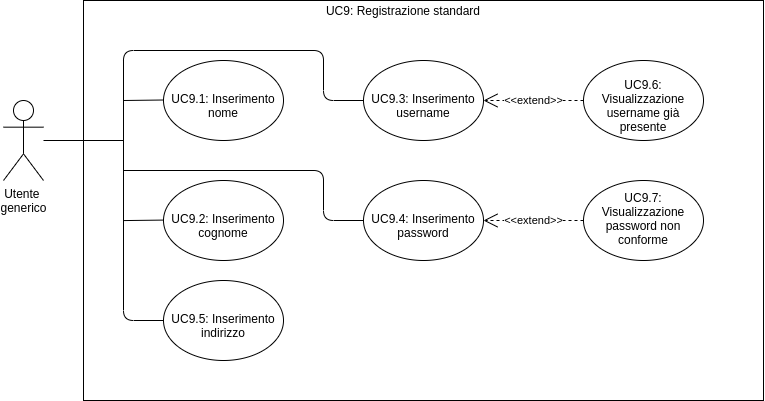
\includegraphics[scale=0.5]{../../../Images/AnalisiRequisiti/UC09.png}
    \centering
\end{figure}
\begin{itemize}
    \item \textbf{Descrizione:} l'utente vuole registrarsi nella piattaforma;
    \item \textbf{Attore Primario:} utente non autenticato;
    \item \textbf{Attore Secondario:} Amazon Cognito;
    \item \textbf{Precondizione:} l'utente non ha un profilo nella piattaforma;
    \item \textbf{Input:} pressione apposito bottone;
    \item \textbf{Postcondizione:} l'utente ha effettuato la registrazione tramite Amazon Cognito.
    \item \textbf{Scenario Principale:}
          \begin{itemize}
              \item un utente arriva per la prima volta nella piattaforma;
              \item si registra attraverso Amazon Cognito, inserendo i seguenti dati:
                    \begin{itemize}
                        \item nome (\hyperref[sec:UC9.1]{\underline{UC9.1}});
                        \item cognome (\hyperref[sec:UC9.2]{\underline{UC9.2}});
                        \item username (\hyperref[sec:UC9.3]{\underline{UC9.3}});
                        \item password (\hyperref[sec:UC9.4]{\underline{UC9.4}});
                        \item ripetizione password.
                    \end{itemize}
              \item l'utente è registrato.
          \end{itemize}
\end{itemize}

\subsubsection{UC9.1: Inserimento nome}
\label{sec:UC9.1}
\begin{itemize}
    \item \textbf{Descrizione:} l'utente inserisce il nome per registrarsi;
    \item \textbf{Attore Primario:} utente generico;
    \item \textbf{Attore Secondario:} Amazon Cognito;
    \item \textbf{Precondizione:} l'utente ha iniziato la registrazione;
    \item \textbf{Input:} stringa con il nome;
    \item \textbf{Postcondizione:} l'utente ha inserito il nome.
\end{itemize}

\subsubsection{UC9.2: Inserimento cognome}
\label{sec:UC9.2}
\begin{itemize}
    \item \textbf{Descrizione:} l'utente inserisce il cognome per registrarsi;
    \item \textbf{Attore Primario:} utente generico;
    \item \textbf{Attore Secondario:} Amazon Cognito;
    \item \textbf{Precondizione:} l'utente ha inserito il nome (\hyperref[sec:UC9.1]{\underline{UC9.1}});
    \item \textbf{Input:} stringa con il cognome;
    \item \textbf{Postcondizione:} l'utente ha inserito il cognome.
\end{itemize}

\subsubsection{UC9.3: Inserimento username}
\label{sec:UC9.3}
\begin{itemize}
    \item \textbf{Descrizione:} l'utente inserisce lo username per registrarsi;
    \item \textbf{Attore Primario:} utente generico;
    \item \textbf{Attore Secondario:} Amazon Cognito;
    \item \textbf{Precondizione:} l'utente ha inserito il cognome (\hyperref[sec:UC9.2]{\underline{UC9.2}});
    \item \textbf{Input:} stringa con lo username;
    \item \textbf{Postcondizione:} l'utente ha inserito lo username.
    \item \textbf{Estensione:} username già presente nel database:
          \begin{itemize}
              \item l'utente può inserire nuovamente lo username \underline{\hyperref[sec:UC38]{UC38}}.
          \end{itemize}
\end{itemize}

\subsubsection{UC9.4: Inserimento password}
\label{sec:UC9.4}
\begin{itemize}
    \item \textbf{Descrizione:} l'utente inserisce la password per registrarsi;
    \item \textbf{Attore Primario:} utente generico;
    \item \textbf{Attore Secondario:} Amazon Cognito;
    \item \textbf{Precondizione:} l'utente ha inserito lo username (\hyperref[sec:UC9.3]{\underline{UC9.3}});
    \item \textbf{Input:} stringa con la password;
    \item \textbf{Postcondizione:} l'utente ha inserito sia la password che la conferma.
    \item \textbf{Scenario Principale:}
          \begin{itemize}
              \item l'utente ha inserito tutti gli altri dati;
              \item l'utente inserisce la propria password;
              \item l'utente inserisce la conferma della password;
              \item l'utente termina la registrazione.
          \end{itemize}
    \item \textbf{Estensione:} la password inserita non è conforme ai requisiti:
          \begin{itemize}
              \item L'utente può reinserire la password rispettando i requisiti \underline{\hyperref[sec:UC39]{UC39}}.
          \end{itemize}
\end{itemize}